\documentclass{article}
\usepackage[utf8]{inputenc}
\usepackage{amstext}
\usepackage{amsmath} 
\usepackage{mathpazo}
\usepackage{graphicx} 
\usepackage{float} 
\usepackage{caption} 
\usepackage{epstopdf} 
\usepackage{hyperref}
\usepackage{varioref} 
\usepackage{fancyref}
\usepackage[section]{placeins} 
\usepackage{perpage}
\usepackage[margin=1in, paperwidth=8.5in, paperheight=11in]{geometry} 
\MakeSorted{figure} 
\usepackage{natbib}
\usepackage{graphicx}
\usepackage{xcolor}
\usepackage{listings}
\usepackage{minted}
\usepackage{subcaption}
\usepackage{eso-pic}
\usepackage{tikz}
\usepackage[american]{circuitikz}
\usepackage[font=small,labelfont=bf]{caption}

\title{ENGR2420 Lab 1 : Resistors and Resistive Networks}
\author{Abigail Fry \\ Anusha Datar \\ Vienna Scheyer}
\date{February 11, 2018}

\begin{document}

\maketitle

\section{Experiment One : Resistance Measurement}
For this experiment, we measured the resistance value of a single 0.25 W resistor by means of reading the printed color codes, a Keithley 2400 SourceMeter\textsuperscript{TM} in resistance mode, and the slope of the linear relationship of the change in voltage across and current through the resistor.

\begin{figure}[H]   
  \centering        
  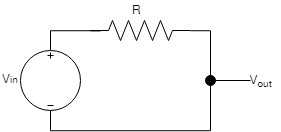
\includegraphics[scale = 0.5]{images/exp1_schematic.jpg}
  \caption{The schematic for the setup we used to measure the resistor value in Experiment One.}   
  \label{fig:circuits_exp1}
\end{figure}

\subsection{Results}
For our first measurement, we noted that the color codes on our resistor corresponded to a value of $402\Omega$. Then, by placing one probe of the SourceMeter\textsuperscript{TM} on each lead of the resistor, we measured a resistance of $401.9 \Omega$. Lastly, we used the SMU to measure the relationship of the change in current depending on a varied voltage; the slope of this line is the resistance of the resistor in Ohms.

\begin{figure}[H]
    \centering
    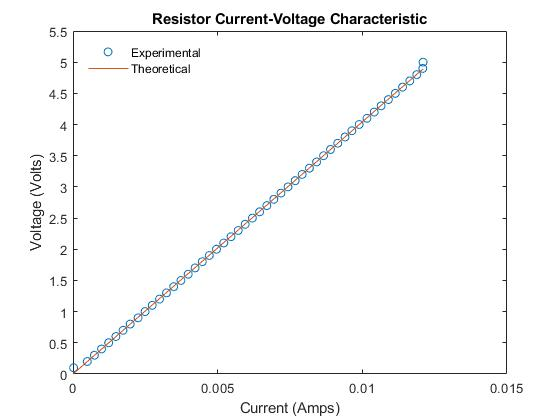
\includegraphics[scale = 0.4]{plot_Ex1.jpg}
    \caption{This figure shows the relationship between input current and and output voltage for the circuit used to determine the resistance.}
    \label{fig:plot_exp1}
\end{figure}

Based on this plot, the resistance is $404.4450 \Omega$.

\subsection{Analysis}

To find the resistance in Ohms based on the current-voltage characteristic of the resistor, we found the slope of the line in Figure 2 using MATLAB's $polyfit$ function. The slope of the best fit line for the experimental data is 404.4450 $\Omega$, so this is the resistance value.

For the SourceMeter\textsuperscript{TM} measurement, we calculated the absolute error as follows:

\begin{center}
    SourceMeter\textsuperscript{TM} Error = $|$Expected - Actual$|$ = $|402\Omega - 401.9\Omega| = 0.1\Omega$
\end{center}

For SMU measurement, we calculated the absolute error of this resistance as follows:

\begin{center}
    SMU Error = $|$Expected - Actual$|$ = $|402\Omega - 404.4450\Omega| = 2.445\Omega$
\end{center}

This translates to 0.025\% error for the SourceMeter\textsuperscript{TM} and a 0.608$\%$ error for the SMU measurement. Both of these are within the $\pm$1$\%$ specified tolerance of this particular resistor.

\subsection{Discussion}
The printed value of the resistor used was 402 $\Omega$ compared with the experimental resistance found using the source meter (401.9 $\Omega$) and the SMU (404.4450 $\Omega$). This resistor has an associated tolerance to allow for minor manufacturing defects of up to 1$\%$.  The difference between the experimental resistance and the expected value for the resistor is within the 1$\%$ error tolerance, but there are other potential causes for the absolute error between values. While the SourceMeter\textsuperscript{TM} has a high internal resistance, it does not have the infinite resistance associated with perfect voltage measurement. The high internal resistance could be the reason the voltage appeared lower than the printed value of the resistor.  Furthermore, the experimental resistance found using the current-voltage plot analyzed a limited set of points to create a line of best fit. The limited sample size likely impacted the resistance calculated from the slope of the line.  

\section{Experiment Two : Resistive Voltage Division}
The second experiment involved using Bourns resistor array chips to explore the effects of small variations in resistor values of a given tolerance and to examine the impacts of creating a voltage divider on the measured resistance. 

We measured the resistance values of each individual resistor in the resistor array using the configuration specified in Experiment 1 in Figure 1. For the voltage divider, we chose to use a 1:1 voltage divider ratio and connected two resistors in series and measured the voltage output at the node in between the two resistors.
\begin{figure}[H]   
  \centering        
  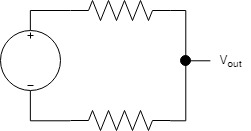
\includegraphics[scale = 0.5]{images/exp2_schematic.jpg}
  \caption{The general configuration used to measure the voltage divider ratio in Experiment 2.}
  \label{fig:exp2}
\end{figure}

\subsection{Results}
First, we used the SourceMeter\textsuperscript{TM} to determine the resistance values of every resistor in two Bourns resistor array chips using the same configuration for resistance measurement specified in Experiment One. These resistances and the absolute error associated with these resistances are listed in the following table. 
\begin{center}
\small\addtolength{\tabcolsep}{-5pt}
    \textbf{Table 1:} Bourns resistor array resistance and percent error values.
    \begin{tabular}{|c|c|c|c|}
        \hline
        Chip 1 Measured Resistance (kΩ) & Chip 1 Percent Error &
        Chip 2 Measured Resistance (kΩ) & Chip 2 Percent Error \\ \hline
        9.935 & 0.65 & 9.937 & 0.63 \\ \hline
        9.936 & 0.64 & 9.930 & 0.7 \\ \hline
        9.928 & 0.72 & 9.930 & 0.7 \\ \hline
        9.934 & 0.66 & 9.937 & 0.63 \\ \hline
        9.940 & 0.6 & 9.949 & 0.63 \\ \hline
        9.937 & 0.63 & 9.954 & 0.46 \\ \hline
        9.940 & 0.6 & 9.949 & 0.51 \\ \hline
        9.935 & 0.65 & 9.944 & 0.56 \\ \hline
    \end{tabular}
\end{center}

We also used the SMU to measure the relationship between the input voltage and the voltage at the central node of a 1:1 voltage divider.
\begin{figure}[H]
    \centering
    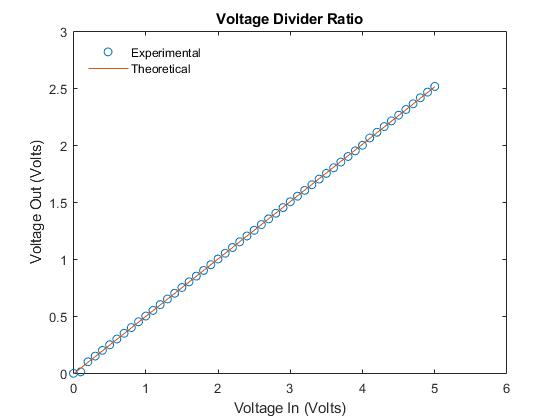
\includegraphics[width=10cm]{plot_Ex2.jpg}
    \caption{This figure shows the relationship between input voltage and and output voltage for the divider circuit in Figure \ref{fig:exp2}}
    \label{fig:ramp}
\end{figure}

\subsection{Analysis}
The specifications of the Bourns resistor array indicate a ±2\% tolerance. The percent errors stated in Table 1 were calculated by dividing the absolute value of the difference between the experimental and theoretical values by the theoretical value. The error values of the resistors are well within the specified tolerance.

Using MATLAB's $polyfit$ function on the voltage and current data points sampled from the SMU, we determined that the slope of the line was 0.5032. This value is a dimensionless ratio and is the difference between the input voltage and the output voltage measure at the node in center of the divider. 
\newline

Since the resistors in this voltage divider circuit are both 10k$\Omega$, the output voltage should be half of the input voltage. This is based on the voltage divider equation

\begin{center}
    $V_{out} = V_{in}\frac{R_2}{R_1 + R_2} = V_{in}\frac{R}{2R} = \frac{1}{2}V_{in}$
\end{center}

In the pre-lab, we learned how to calculate the tolerance of a resistive divider ratio. We used resistors 1 and 2 on the Bourns resistor chip for this voltage divider circuit. Substituting the experimentally measured values for $R_1$ and $R_2$ into the divider ratio tolerance equation yields the following expression.

\begin{center}
    $\frac{R_2 \delta R_1 - R_1 \delta R_2}{(R_1 + R_2)^2} = \frac{(9.936)(0.0036) - (9.935) (0.0064)}{(9.935 + 9.936)^2} = \pm 7.044 x 10^{-5}$ 
\end{center}

When we calculate the actual error based on the values for $V_{out}$ and $V_{in}$ we get the error associated with our circuit configuration. The absolute error of the voltage divider is a dimensionless expression because the units ($\Omega$) cancel out.

\begin{center}
    $|$Expected $- \frac{V_{out}}{V_{in}}| = |0.5 - 0.5032| = 0.0032$
\end{center}
This difference is orders of magnitude larger than our expected tolerance. 

\subsection{Discussion}
The actual divider ratio is larger than the theoretical divider ratio by a value that exceeds the tolerance associated with the resistor values themselves. This implies that while variations in the resistor values could certainly be involved in generating error, it is not the sole source of discrepancy. Other possible problematic factors include noise associated with the breadboard and the wire connections - these values could have easily distorted the output, causing the experimental value to diverge. Furthermore, this particular divider ratio was calculated by means of sampling points during a voltage sweep - because of the limited quantity of points available, the line of best fit might not completely accurately represent the ratio. Because the voltage divider ratio is a ratio, it is likely that the bias associated with the actual voltage measurement (and the internal resistance of the measurement device) had less of an impact than in other cases. 

\section{Experiment 3 : Resistive Current Division}

For this section of the lab, we made a current divider circuit and measured the output current. We chose to use resistors in a 1:1 ratio. 
\begin{figure}[H]
    \centering
    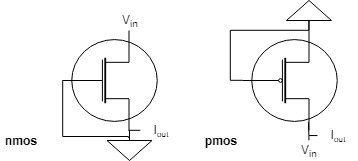
\includegraphics[scale=0.5]{images/exp3_schematic.jpg}
    \caption{Schematic diagram for current divider ratio circuit.}
    \label{fig:exp3}
\end{figure}


\subsection{Results}
To record the value of the current divider ratio, we placed our SMU in series with the circuit following the second of two parallel resistors as specified in Figure 5 and measured the value of the current through this point during an input current sweep.
\begin{figure}[H]
    \centering
    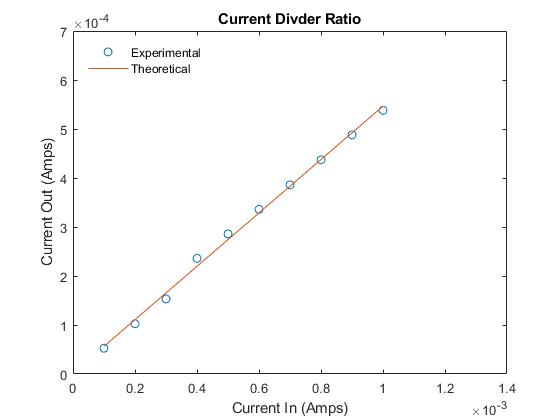
\includegraphics[width=10cm]{plot_Ex3.jpg}
    \caption{This figure shows the relationship between input current and and output current for the divider circuit in Figure \ref{fig:exp3}.}
    \label{fig:ramp}
\end{figure}
\subsection{Analysis}
We found the slope using MATLAB's $polyfit$ function on the experimental data.  The slope of the best fit line is 0.5446.
This value is a dimensionless ratio and is the difference between the input current and the output current in a node in the divider. 
\newline
Since we used two resistors of the same resistance, the current divider should theoretically have divided the current exactly in half. We had a 0.89\% error in the slope of our experimental data.
\newline
Again, we can apply the divider ratio tolerance equation from the prelab assignment. We again resistors 1 and 2 on the Bourns resistor chip for this current divider circuit. Substituting the experimentally measured values for $R_1$ and $R_2$ into the divider ratio tolerance equation yields the following expression.

\begin{center}
    $\frac{R_2 \delta R_1 - R_1 \delta R_2}{(R_1 + R_2)^2} = \frac{(9.936)(0.0036) - (9.935) (0.0064)}{(9.935 + 9.936)^2} = \pm 7.044 x 10^{-5}$ 
\end{center}

When we calculate the actual error based on the values for $V_{out}$ and $V_{in}$ we get the (dimensionless) error associated with our circuit configuration. 

\begin{center}
    $|$Expected $- \frac{V_{out}}{V_{in}}| = |0.5 - 0.5446| = 0.0446$
\end{center}
This difference is orders of magnitude larger than our expected tolerance. 

\subsection{Discussion}
This ratio is also much higher than expected. While the differences in resistor tolerances can impact the measured value, the actual discrepancy is much larger than the maximum discrepancy that can be attributed to them. This implies that there are other sources of error as well. Like with the voltage divider, the difference could be associated with noise in the breadboard and connections and the limited sample of data points taken. Because the current divider ratio is a ratio, it is likely the bias associated with the actual current measurement (and the internal resistance of the measurement device) had less of an impact than in other cases. 
\newline
Another issue could relate to our SMU itself; during Experiment Four, we had several issues measuring current accurately and eventually resigned to using a multimeter for data collection. Therefore, it is definitely possible that there are measurement errors associated with the ratio. 

\section{Experiment 4 : R-2R Ladder Network}
For the fourth experiment, we created an R-2R ladder network with four 2R branches and then measured the current at various points along the ladder network.

\begin{figure}[H]
    \centering
    \includegraphics[width=10cm]{images/exp4_overview.png}
    \caption{Overview diagram of the R-2R ladder network.}
    \label{fig:ramp}
\end{figure}

To create this circuit using the Bourns resistor array chips, we used two chips of eight equal resistors each to create a circuit with the necessary connections and resistance ratios.

\begin{figure}[H]
    \centering
    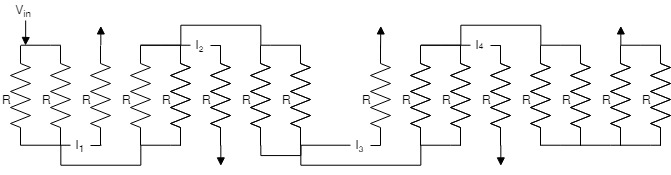
\includegraphics[width=14cm]{images/exp4_schematic.jpg}
    \caption{The schematic used in the experimental set up for the R-2R ladder network using the Bourns resistor chip.}
    \label{fig:ramp}
\end{figure}

\subsection{Results}
We measured the value of the current at the four points noted in the schematic with an input voltage of 5 Volts and with an input voltage of 3.3 Volts.
\begin{center}
\textbf{Table 2:} Current data collected at nodes 1-4  for 3.3 and 5 volts. 

\small\addtolength{\tabcolsep}{-5pt} 
    \begin{tabular}{|c|c|c|}
        \hline
          & Input: 5V & Input: 3.3V \\ \hline
        Current at point 1 (mA) :& 0.25 & 0.16\\ \hline
        Current at point 2 (mA) :& 0.12 & 0.08\\ \hline
        Current at point 3 (mA) :& 
       0.06 & 0.04\\ \hline
        Current at point 4 (mA) :& 
        0.03 & 0.02\\ \hline
    \end{tabular}
\end{center}

The plot in Figure \ref{exp4} shows the theoretical values we calculated and experimental data we collected for the ladder network. The x-axis shows the measurement locations in the circuit (corresponding to the $I_n$ points in Figure 8) and the y-axis shows the output current in mA.

\begin{figure}[H]
    \centering
    \includegraphics[width=14cm]{Exp4_plot.png}
    \caption{The plotted theoretical and experimental data for the R-2R ladder network.} \label{exp4}
    \label{fig:ramp}
\end{figure}

The data is plotted on semi-logarithmic axes. This shows that the exponential behaviour of the current division pattern is linear in a logarithmic framework.

\subsection{Analysis}
We used the following formula that we derived in the prelab assignment to calculate the theoretical currents at the four points labeled in the schematic. 

\begin{center}
    $I_N = \frac{(\frac{V_{in}}{R})}{2^{N}}$
\end{center}

Based on this equation, we calculated the theoretical currents through each of the 2R branches in the resistor ladder circuit, indexing from left to right. The following table shows theoretical values when the inputs are 3.3V and 5V.

\begin{center}
\textbf{Table 3:} Theoretical currents through the four 2R branches in the ladder network.
\small\addtolength{\tabcolsep}{-5pt}
    \begin{tabular}{|c|c|c|}
        \hline
          & Input: 5V & Input: 3.3V \\ \hline
        Current at point 1 (mA) & 0.25 & 0.165\\ \hline
        Current at point 2 (mA) & 0.125 & 0.0825\\ \hline
        Current at point 3 (mA) & 0.0625 & 0.04125\\ \hline
        Current at point 4 (mA) & 0.03125 & 0.020625\\ \hline
    \end{tabular}
\end{center}

When measuring the current values with the SMU, we were unable to record data which was compatible with either the theoretical values or the theoretical ratio between the values at successive points. We recorded a much larger input current than expected and varied (and asymmetric) decreases in current at each point. As a result, we chose to measure current using a multimeter instead, which yielded measurements significantly closer to the expected values and more consistent with expected relationships between points. To record data points, we replaced the wire at each point with the two multimeter leads. 
Because the multimeter we had access to only displayed two significant figures for the given range of values, we were limited in our ability to make precise measurements. However, we were still able to examine the ratio of the values from node to node. 

The table below shows the percent errors errors for all the points in the R-2R ladder network current measurement graph. The most prominent source of error in these measurements is our lack of significant figures.

\begin{center}
\textbf{Table 4:} Experimentally measured currents through the four 2R branches in the ladder network.
\small\addtolength{\tabcolsep}{-5pt}
    \begin{tabular}{|c|c|c|c|c|} \hline
          & Input: 5V & \% Error & Input: 3.3V & \% Error \\ \hline
        Current at point 1 (mA) & 0.25 & 0 & 0.16 & 3\\ \hline
        Current at point 2 (mA) & 0.12 & 4 & 0.08 & 3 \\ \hline
        Current at point 3 (mA) & 0.06 & 4  & 0.04 & 3 \\ \hline
        Current at point 4 (mA) & 0.03 & 4  & 0.02 & 3\\ \hline
    \end{tabular}
\end{center}

\subsection{Discussion}

The discrepancy between the theoretical and experimental values is higher than expected.  A potentially large factor in this error was from the measurement technique.  Due to challenges with the SMU, we tested and recorded the current values using a multimeter. The lack of significant figures displayed by the meter made it impossible to accurately record the current to the depth necessary to rigorously examine the accuracy of the measured ratio. This is because the theoretical values, which we calculated using the current divider equation and Ohms law, were not constrained to the 2 significant figures given by the multimeter. Another likely factor is the wiring and connections associated with the circuit: there are a multitude of fairly loopy and possibly insecure connections that make up the ladder. These likely could have caused interference via inductance or noise due to poor connections.

Despite the lack of precision in our data collection, we could still see that these current measurements varied in position as we expected. In other words, the experimental measurements followed the trend that we predicted in which the current is halved at each node in the ladder network.

\end{document}
